\begin{figure}[htbp]
\centering
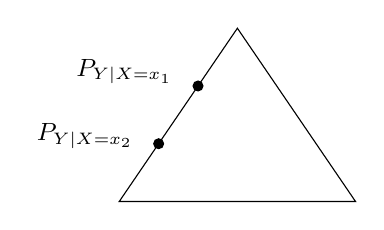
\begin{tikzpicture}[x=1cm,y=1cm]
 \draw (0,0)--(1.5,2.2)--(3,0)--cycle;
 \fill (1,1.466667) circle[radius=2pt];
 \fill (.5,.733333) circle[radius=2pt];
 \node[left,font=\small] at (.8,1.65) {$P_{Y\mid X=x_1}$};
 \node[left,font=\small] at (.3,.83) {$P_{Y\mid X=x_2}$};
\end{tikzpicture}
\caption{非纯条件分布的另一个例子：连接$P_{Y\mid X=x_1}$与$P_{Y\mid X=x_2}$的线段，可以延长而不离开单纯形。}
\end{figure}
